%-------------------------------------------------------------------------------
%                      Template Naskah TA Skema Skripsi
%             Format berdasarkan format yang disepakati di Fakultas
% 						(c) @RikieKartadie 2025
%-------------------------------------------------------------------------------

%Template pembuatan naskah TA Skema skripsi.
\documentclass[duaspasi]{utdiskripsi}

%%%==== bagian ini untuk sibfile, halpdf, dan lscape
\usepackage{subfiles} %ngurusi anak file
\usepackage{pdfpages} %nyisipkan file pdf
\usepackage{lscape}
\usepackage[shortlabels]{enumitem}
\usepackage{multirow}
\usepackage{multicol}
\usepackage[center]{caption}
\usepackage{longtable}
\usepackage{booktabs}
%anda dapat tambahkan paket seperti kebutuhan anda
%-----------------------------------------
%%%%buat cell color
\usepackage{color}
\usepackage{colortbl}
\definecolor{abu}{cmyk}{0,0,0,0.06}

%\addbibresource{daftar-pustaka}

%Untuk prefiks pada daftar gambar dan tabel
\usepackage[titles]{tocloft}
\renewcommand\cftfigpresnum{Gambar\  }
\renewcommand\cfttabpresnum{Tabel\   }

%=================METADATA DARI PDF =================
\newcommand{\AuthorName}{Rikie Kartadie} 	% <=== Rubah kenamamu
\newcommand{\ThesisTitle}{Judul TA Skema Skripsi} %<=== Rubah ke judul TA mu
\newcommand{\ThesisSubject}{Subjek TA mu} %<=== Rubah ke Subjek/fokus TA mu
\newcommand{\Supervisor}{Dr. Budi Santosa} %<=== Nama pembimbingmu
\newcommand{\ThesisKeywords}{Keyword1, Keyword2, Keyword3, Keyword4, Keyword5} %<== Tulis Keywordmu 

%%%%---Bagian ini Jangan di rubah ----
\usepackage{etoolbox}
\makeatletter
\@ifpackageloaded{hyperref}{
	\hypersetup{
		pdfauthor={\AuthorName},
		pdftitle={\ThesisTitle},
		pdfsubject={\ThesisSubject},
		pdfkeywords={\ThesisKeywords},
		unicode,
		pdfborder={0 0 0},
		bookmarksnumbered=true,
		bookmarksopen=true,
		bookmarksopenlevel=1,
		colorlinks=false,
		pdfnewwindow=true,
		pdfpagelayout=SinglePage,
		pdfdisplaydoctitle=true
	}
}{
	\usepackage{hyperref}
	\hypersetup{
		pdfauthor={\AuthorName},
		pdftitle={\ThesisTitle},
		pdfsubject={\ThesisSubject},
		pdfkeywords={\ThesisKeywords},
		unicode,
		pdfborder={0 0 0},
		bookmarksnumbered=true,
		bookmarksopen=true,
		bookmarksopenlevel=1,
		colorlinks=false,
		pdfnewwindow=true,
		pdfpagelayout=SinglePage,
		pdfdisplaydoctitle=true
	}
}%
%========================================================


\newlength{\mylenf}
\settowidth{\mylenf}{\cftfigpresnum}
\setlength{\cftfignumwidth}{\dimexpr\mylenf+2em}
\setlength{\cfttabnumwidth}{\dimexpr\mylenf+2em}
\usepackage[labelfont=bf]{caption}
\usepackage{caption}
\usepackage{subcaption}
\hyphenation{
	soft-ware 										
	di-la-ku-kan 
	di-la-kukan 
	me-nam-bah-kan
	meng-gu-na-kan
	re-le-van
	di-tam-pil-kan
} %<===tambahkan pemenggalan kata bahasa indonesia di file ini.

%-----------------------------------------------------------------
%Disini awal masukan untuk data TA skema skripsi mu
%-----------------------------------------------------------------
\titleind{INI JUDUL ANDA TIDAK LEBIH DARI 12 KATA DAN TEMPLATE INI MENGGUNAKAN \LaTeX}

\fullname{NAMA ANDA}

\idnum{123456789} %<== INI NIM ANDA

\Semester{8 (Delapan)} %<====Semester pada saat Ujian Tugas Akhir 

\TAakademik {Genap 2024/2025} %<==Tahun Akademik saat Ujian Tugas Akhir

\approvaldate{3 Februari 2025}% <==ini tanggal pengesahan

\tanggalujian{20 Februari 2025} %<=== INI TANGGAL UJIAN ANDA

\degree{Sarjana Komputer}

\yearsubmit{2025}

\program{Sarjana}

%PRODI
\dept{Sistem Informasi}
\kaprodi{Prof. MeiMei Upin Ipin,  PhD.} %<===Kaprodi anda
\nidnkapro{134679852} %<==NIDN KAPRODI

%PEMBIMBING
\firstsupervisor{Prof. Deborah Kurniawati,  PhD.} %<===Nama Pemboimbing anda
\firstnip{0501120004} %<== INI NIDN DOSPEM ANDA

%PENGUJI
\pengujipertama{Prof. Dini Fakta Sari, PhD} %<====== INI PENGUJI I ANDA
\secondnip{9876543210} %<===== INI NIDN PENGUJI I
\pengujikedua{Prof. Mahfud MD} % <===== INI PENGUJI 2 ANDA
\nidnpengdua{0123456789} %<== INI NIDN PENGUJI 2


%-----------------------------------------------------------------
%Disini akhir masukan untuk data proposal skripsi
%-----------------------------------------------------------------

\begin{document}

\cover
\ajuanpage
\halsetuju
\approvalpage
%\approvalpage

%==================PERNYATAAN KEASLIAN=========
\bebasplagiat
\makeatletter
\let\kaprodi\@kaprodi
%\let\kajur\@kajur
\let\pembimbingA\@firstsupervisor
%\let\pembimbingB\@secondsupervisor
\let\jurusan\@dept
\let\sarjana\@degree
\let\fullname\@fullname
\let\idnum\@idnum
\let\titleind\@titleind
\let\tglsetuju\@approvaldate
\let\faculty\@faculty
\makeatother
%\hyphenation{mau-pun pa-sien Yog-ya-kar-ta YOGYA-KAR-TA nasio-nal na-sio-nal}

%------------------------------------

%------------------------------------
% Mulai kata pengantar di bawah ini
% -----------------------------------
\vspace{2.5cm}

Dengan ini saya menyatakan bahwa naskah Tugas Akhir ini belum pernah diajukan untuk memperoleh gelar \sarjana~di suatu Perguruan Tinggi, dan sepanjang pengetahuan saya tidak terdapat karya atau pendapat yang pernah ditulis atau diterbitkan oleh orang lain, kecuali yang secara sah diacu dalam naskah ini dan disebutkan dalam daftar pustaka.


\begin{tabular}{p{5.7cm}l}
	&\\
	&\\
	&Yogyakarta, \tglsetuju\\
	
	&	\\
	&	\\
	&	\\
	&	\multicolumn{1}{c}{\bfseries \underline{\fullname}}\\
	& \multicolumn{1}{c}{NIM~:~\idnum}\\
\end{tabular}

%----------------------------------------------

%-----------------------------------------------------------------
%Disini awal masukan Acknowledment
%-----------------------------------------------------------------
\acknowledgment
%Persembahan
\vspace*{1cm}
%===========================
% Mulai dari sini
%===========================
Berisi persembahan kepada orang tertentu, misalnya orang tua, sahabat, dan lain-lain. Pengisian halaman ini dibatasi pada kata-kata ataupun kalimat. Tidak dibenarkan untuk menghiasinya dengan gambar-gambar tertentu. Pada bagian tengah bawah diketik nomor halaman dengan angka Romawi kecil.

%-----------------------------------------------------------------
%Disini awal masukan untuk Prakata
%-----------------------------------------------------------------
\preface
%PRAKATA

\makeatletter
\vspace*{1cm}

Halaman ini memuat pengantar tentang penelitian dan ucapan terima kasih mahasiswa kepada mereka yang telah membantunya selama pendidikan. Kalimat- kalimatnya pendek, terdiri dari beberapa alinea, namun tidak lebih dari dua halaman.

Di akhir teks dicantumkan kata-kata kota penerbitan, bulan dan tahun, yang diikuti kata Penulis di kanan bawah. Di bagian tengah bawah diketik nomor halaman dengan angka Romawi kecil.

conoth bagian akhir adalah sebagai berikut 

%-----------bag akhiir
\vspace{1cm}
\begin{tabular}{p{7.5cm}c}
	&Wassalamu'alaikum Wr. Wb.\\
	&Yogyakarta, Agustus 2025\\
	&\\&\\
	&\textbf{Penulis}
\end{tabular} %<== perbaiki /rubah pada file ini 

%-----------------------------------------------------------------
%Disini akhir masukan untuk muka skripsi
%-----------------------------------------------------------------
\tableofcontents
\addcontentsline{toc}{chapter}{DAFTAR ISI}
\listoftables
\addcontentsline{toc}{chapter}{DAFTAR TABEL}
\listoffigures
\addcontentsline{toc}{chapter}{DAFTAR GAMBAR}
\listoflistings
\addcontentsline{toc}{chapter}{DAFTAR MODUL PROGRAM}


%-----------------------------------------------------------------
%Daftar Singkatan [Optional]
%-----------------------------------------------------------------
%\singkatan
\noindent

	%-----------------------------------------------------------------
%Disini awal masukan Intisari
%-----------------------------------------------------------------
%bahasa ina
\begin{abstractind}
	%intisari ina
INI ADALAH INTISARI
Lorem ipsum dolor sit amet, consectetur adipisicing elit, sed do eiusmod tempor incididunt ut labore et dolore magna aliqua. Ut enim ad minim veniam, quis nostrud exercitation ullamco laboris nisi ut aliquip ex ea commodo consequat. Duis aute irure dolor in reprehenderit in voluptate velit esse cillum dolore eu fugiat nulla pariatur. Excepteur sint occaecat cupidatat non proident, sunt in culpa qui officia deserunt mollit anim id est laborum.

Sed ut perspiciatis unde omnis iste natus error sit voluptatem accusantium doloremque laudantium, totam rem aperiam, eaque ipsa quae ab illo inventore veritatis et quasi architecto beatae vitae dicta sunt explicabo. Nemo enim ipsam voluptatem quia voluptas sit aspernatur aut odit aut fugit, sed quia consequuntur magni dolores eos qui ratione voluptatem sequi nesciunt.


\bigskip
\noindent
\textbf{Kata kunci :} \emph{wireless sensor network}, \emph{Internet Protocol}, WiFi, interoperabilitas.

\end{abstractind}

\begin{abstracteng}
	
\emph{
	INI INTISASRI BAHASA INGGRIS Lorem ipsum dolor sit amet, consectetur adipisicing elit, sed do eiusmod tempor incididunt ut labore et dolore magna aliqua. Ut enim ad minim veniam, quis nostrud exercitation ullamco laboris nisi ut aliquip ex ea commodo consequat. Duis aute irure dolor in reprehenderit in voluptate velit esse cillum dolore eu fugiat nulla pariatur. Excepteur sint occaecat cupidatat non proident, sunt in culpa qui officia deserunt mollit anim id est laborum.}

\emph{Sed ut perspiciatis unde omnis iste natus error sit voluptatem accusantium doloremque laudantium, totam rem aperiam, eaque ipsa quae ab illo inventore veritatis et quasi architecto beatae vitae dicta sunt explicabo. Nemo enim ipsam voluptatem quia voluptas sit aspernatur aut odit aut fugit, sed quia consequuntur magni dolores eos qui ratione voluptatem sequi nesciunt.}

\bigskip
\noindent
\textbf{\emph{Keywords :}} \emph{wireless sensor network, Internet Protokol, WiFi, interoperability}.

\end{abstracteng}
%-----------------------------------------------------------------
%Disini akhir masukan Intisari
%-----------------------------------------------------------------

%-----------------------------------------------------------------
%Disini awal masukan untuk Bab
%-----------------------------------------------------------------
%!TEX root = ./template-skripsi.tex
% Gunakan \cite{citekey} untuk IEEE Style
% Gunakan \parencite{citekey} untuk APA Stle
%-------------------------------------------------------------------------------
% 								BAB I
% 							LATAR BELAKANG
%-------------------------------------------------------------------------------

\chapter{PENDAHULUAN}

\section{Latar Belakang}
Berisi argumen atau alasan berdasarkan fakta atau sumber-sumber penelitian sebelumnya (bukan opini dari penulis), sehingga perlunya dibuat penelitian ini. Uraian dimulai dengan hal yang unik, fakta, masalah dan pendapat yang mendasari penelitian. Diuraikan juga alasan-alasan teoritis dan praktis perlunya penelitian ini dilakukan dan bagaimana masalah tersebut dipecahkan.\parencite{abdillahfudholi2024}.

\section{Rumusan Masalah}
Berbekal latar belakang dan kerangka pikir, masalah yang diteliti dapat dirumuskan. Masalah yang dirumuskan harus jelas dan fokus pada kata kunci utama yang unik. Dalam merumuskan masalah, deskripsi lokasi studi terutama keunikannya sudah termasuk dalam pertimbangan. Untuk memperjelas perumusan masalah, dapat juga dibuat beberapa pertanyaan yang hendak dijawab dalam penelitian itu. Dalam uraian harus tercakup pendekatan yang digunakan dalam perumusan masalah. Untuk membantu mengikuti alur pikir secara skematis, dapat juga dibuat bagan alir kerangka proses dan rumusan masalah serta pencapaian tujuan penelitian\parencite{adha2021}.


\section{Ruang Lingkup}
Berisi uraian yang menjelaskan kompleksitas atau lingkup obyek yang diteliti. Ruang lingkup berisi deskripsi pekerjaan yang akan dilakukan (bukan apa yang tidak dikerjakan). Contohnya variabel, kriteria, ciri, cara pengujian, metode, model dan lain-lain. Disajikan dalam bentuk pointer.


\section{Tujuan Penelitian}
Menjelaskan tujuan yang akan dicapai sebagai upaya pemecahan masalah yang dijelaskan dalam latar belakang. Gunakan kata kerja yang hasilnya dapat diukur, bukan menunjukan syarat kelulusan.


\section{Manfaat Penelitian}
Menjelaskan manfaat atau kegunaan hasil penelitian bagi kepentingan pengembangan ipteks, pertimbangan dalam mengambil kebijakan, kepentingan profesi maupun masyarakat pada umumnya.

Jika ada bagian yang berbentuk enumerate maka dapat mencontoh kode ini:
\begin{enumerate}[noitemsep]
	\item ini bagian yang diberi list
	\item ini nomor yang diberi list
	\item ini nomor yang diberi list lain
\end{enumerate}

\section{Sistematika Penulisan}
Keterangan masing-masing isi bab secara ringkas. Gambaran umum tiap bab akan diterangkan pada subbab ini, dengan cara deskriptif, bukan dalam bentuk daftar. Jangan pindahkan Daftar Isi ke sini.\\
\noindent
\textbf{BAB I : PENDAHULUAN}

Pada bab ini dijelaskan latar belakang, rumusan masalah, batasan, tujuan, manfaat, keaslian penelitian, dan sistematika penulisan.\\

\noindent
\textbf{BAB II : TINJAUAN PUSTAKA DAN DASAR TEORI}

Pada bab ini dijelaskan teori-teori dan penelitian terdahulu yang digunakan sebagai acuan dan dasar dalam penelitian.\\

\noindent
\textbf{BAB III : METODE PENELITIAN}

Pada bab ini dijelaskan metode yang digunakan dalam penelitian meliputi langkah kerja, pertanyaan penilitian, alat dan bahan, serta tahapan dan alur penelitian.\\

\noindent
\textbf{BAB IV :IMPLEMENTASI DAN PEMBAHASAN}

Pada bab ini dijelaskan implementasi penelitian dan pembahasannya.\\

\noindent
\textbf{BAB V : PENUTUP }

Pada bab ini ditulis kesimpulan akhir dari penelitian dan saran untuk pengembangan penelitian selanjutnya.\\

% Baris ini digunakan untuk membantu dalam melakukan sitasi
% Karena diapit dengan comment, maka baris ini akan diabaikan
% oleh compiler LaTeX.
\begin{comment}
\bibliography{daftar-pustaka}
\end{comment}


%!TEX root = ./template-skripsi.tex
% Gunakan \cite{citekey} untuk IEEE Style
% Gunakan \parencite{citekey} untuk APA Stle
%-------------------------------------------------------------------------------
%                            BAB II
%               TINJAUAN PUSTAKA DAN DASAR TEORI
%-------------------------------------------------------------------------------

\chapter{TINJAUAN PUSTAKA DAN DASAR TEORI}                

\section{Tinjauan Pustaka}
  Pustaka yang digunakan dalam bab ini ialah acuan primer; diutamakan artikel berkala ilmiah yang relevan dengan bidang yang diteliti, terkini, dan asli (\textit{state of the art}). Diktat dan buku ajar tidak termasuk acuan primer. Tinjauan pustaka memuat kajian singkat, jelas, dan sistematis tentang kerangka teoretis, kerangka pikir, temuan, prinsip, asumsi, dan hasil penelitian yang relevan yang melandasi masalah penelitian atau gagasan guna menggali pemahaman mengenai masalah penelitian dan pemecahan masalahnya. Oleh karena itu, dari tinjauan pustaka harus dapat diturunkan kerangka pikir, hipotesis penelitian, dan metode penelitian. Acuan yang relevan harus dimanfaatkan untuk membahas temuan yang dituangkan kemudian dalam Pembahasan. Kajian pustaka tidak sekadar berisi informasi umum seperti definisi, tetapi berisi informasi dasar yang berkaitan dengan inti penelitian. Kumpulan pustaka yang relevan dan mutakhir membantu penulis memahami perbedaan penelitiaannya dengan penelitian sebelumnya. Kumpulan pustaka yang memadai pasti akan meningkatkan kepercayaan diri penulis sewaktu memilih metode, melaksanakan penelitian, dan menyusun argumentasi dalam bab Pembahasan. Pustaka tidak boleh disitasi secara ekstensif, tetapi ditelaah dan diulas. Setiap pustaka yang diacu harus dicantumkan dalam Daftar Pustaka. Minimal memuat 5 artikel yang terpublikasikan dalam jurnal atau \textit{proceeding} \parencite{affum2021}.

\section{Landasan Teori}
  \subsection{\LaTeX}
Berisi tentang uraian, penjelasan, definisi, pengertian dasar dan ulasan yang didapat dari berbagai sumber atau referensi yang telah dipublikasikan dalam media cetak maupun elektronik (buku teks, artikel, dan lain-lain) serta terkait dengan topic skripsi. Setiap pustaka yang diacu harus dicantumkan dalam Daftar Pustaka \parencite{alden2020}.

Untuk gambar dapat dilihat di Gambar~\ref{wsn}. Pastikan gambar telah anda sebutkan didalam teks, jangan menuliskan \textbf{"Seperti terlihat pada Gambar di bawah atau di atas ini..."} namun tulislah \textbf{"Seperti terlihat pada Gambar~\ref{wsn} berikut."}.


      \begin{figure}[H]
        \centering
          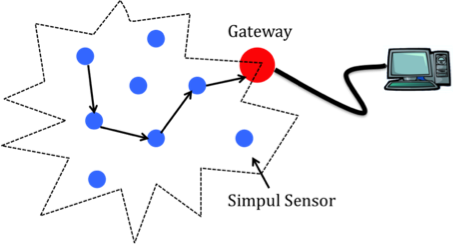
\includegraphics{gambar/wsn}
          \caption{Jaringan sensor nirkabel.}
          \label{wsn}
      \end{figure}


  \subsection{Sublime Text}
    Et affert civibus has. Has ne facer accumsan argumentum, apeirian hendrerit persequeris pro ex. Suscipit vivendum sensibus mea at, vim ei hinc numquam, at dicit timeam dissentiet mel. At patrioque intellegebat sea, error argumentum dissentias sea in.

    Quo no atqui omnesque intellegat, ne nominavi argumentum quo. Eum ei purto oporteat dissentiet, soleat utamur an sit. Et assum dicam interpretaris quo. Cetero alterum ea vel, no possit alterum utroque nec. His fuisset quaestio ad. Has eu tritani incorrupte consequuntur, esse aliquip nec ne \parencite{basconcillo2023}.
    
    
 \subsection{Aturan Penulisan}
   Ketentuan umum penulisan Laporan Skripsi:
   \begin{enumerate}[noitemsep,label=\alph*.]
   	\item   Laporan skrispsi harus dicetak (tidak boleh bolak-balik) pada kertas HVS 70 g/m2, berukuran kuarto atau A4 (21 cm x 28 cm), dan dijilid rapi dengan menggunakan sampul laminasi kertas buffalo berwarna putih.
   	\item Naskah lengkap laporan skripsi disusun dalam bahasa Indonesia yang baku, sesuai dengan ketentuan ejaan bahasa Indonesia yang disempurnakan. Apabila penulisan dalam bahasa Inggris, pedoman penulisan ejaan dan tata-bahasa mengikuti sistem spelling dan grammar berdasarkan tipe US/British English terkait dengan software yang digunakan.
   	\item Semua kalimat ditulis menggunakan tata bahasa baku. Penggunaan kata ganti orang dihindari (digunakan kalimat pasif) dan sedapat mungkin menggunakan istilah Indonesia. Apabila, karena sesuatu hal, terpaksa harus menggunakan istilah asing atau istilah daerah, istilah tersebut harus ditulis miring secara konsisten.
   	\item Dalam penulisan usulan penelitian atau tugas akhir, sebaiknya digunakan kalimat atau alinea penyambung antara definisi/teorema yang satu dengan definisi/teorema yang lain, sehingga alur isi usulan penelitian atau tugas akhir menjadi jelas. Hindari penulisan yang hanya mendaftar definisi, teorema dan lain-lainnya.
   \end{enumerate}
  
   Beberapa ketentuan tata tulis berikut perlu diperhatikan dalam penulisan usulan penelitian atau tugas akhir:
   \begin{enumerate}[noitemsep]
   	\item   Kata hubung, misalnya “maka”, “sehingga”, “sedangkan” tidak boleh digunakan sebagai awal suatu kalimat.
   	\item Penerjemahan kata “where”, “when”, dan “of” dalam bahasa Inggris tidak selalu menjadi kata “di mana”, “ketika”, dan “dari” dalam bahasa Indonesia, tetapi harus diterjemahkan/ diartikan dengan tepat, sesuai dengan bahasa Indonesia baku.
   	\item Perlu diperhatikan bahwa penulisan “ke” dan “di” sebagai awalan, harus dibedakan dengan penulisan “ke” dan “di” sebagai kata depan.
   	\item Pemenggalan kata harus dilakukan secara cermat, sesuai dengan kaidah penulisan Bahasa Indonesia yang benar.
   	\item Bilangan yang mengawali suatu kalimat harus dieja, misalnya : Sepuluh ekor tikus.
   	\item Simbol atau rumus tidak boleh berada di awal kalimat.
   	\item Tanda baca dan penulisan anak kalimat mengikuti EYD.
   \end{enumerate}
  

% Baris ini digunakan untuk membantu dalam melakukan sitasi
% Karena diapit dengan comment, maka baris ini akan diabaikan
% oleh compiler LaTeX.
\begin{comment}
\bibliography{daftar-pustaka}
\end{comment}


%!TEX root = ./template-skripsi.tex
% Gunakan \cite{citekey} untuk IEEE Style
% Gunakan \parencite{citekey} untuk APA Stle
%-------------------------------------------------------------------------------
%                            BAB III
%               		METODE PENELITIAN
%-------------------------------------------------------------------------------

\chapter{METODE PENELITIAN}
Bagian ini menyajikan secara lengkap setiap langkah eksperimen yang dilakukan dalam penelitian menggunakan\textbf{ bentuk kalimat pasif} yang antara lain meliputi:

\section{Bahan/Data} 
Semua bahan/data yang digunakan dikelompokkan sesuai fungsinya berdasarkan kebutuhan analitis dan teknis. Pastikan 1 alenia megandung lebih dari 2 kalimat utuh.

\section{Peralatan} 
Semua peralatan yang digunakan untuk menjalankan penelitian harus disebutkan dan diuraikan dengan jelas dan apabila perlu (terutama peralatan yang dirancang khusus) dapat disertai dengan bagan dan keterangan secukupnya. Peralatan terdiri dari hardware dan software. Hardware yang diuraikan adalah peralatan yang mendukung implementasi dan pengujian. Software merupakan perangkat lunak yang digunakan pada penelitian, dilengkapi dengan versi dan kegunaan. Untuk instrumentasi khusus merk dan tipe/spesifikasi peralatan harus dicantumkan, sedangkan kondisi pengoperasian disajikan pada bagian lain yang sesuai.

\section{Prosedur dan Pengumpulan Data} 
Pada bagian ini, variabel, prosedur, organisasi dan lokasi yang akan dipelajari serta data yang akan dikumpulkan diuraikan dengan jelas, termasuk sifat, satuan dan kisarannya. Untuk pengujian dan pengolahan data diperlukan perancangan dan pengembangan sistem.

\section{Analisis dan Rancangan Sistem} 
Pada bagian ini diuraikan analisis sistem dijelaskansecara diskriptif dan dilengkapi dengan bagan. Selain itu juga diuraikan kebutuhan sistem yang meliputi kebutuhan fungsional, kebutuhan non fungsional sistem. Rancangan sistem meliputi rancangan arsitektur sistem atau gambaran umum sistem, rancangan proses, rancangan prosedural, rancangan data, dan rancangan user interface. Bebarapa kakas yang dapat digunakan antara lain Flowchart, DAD, ERD, normalisasi,UML, dll.

	
% Baris ini digunakan untuk membantu dalam melakukan sitasi
% Karena diapit dengan comment, maka baris ini akan diabaikan
% oleh compiler LaTeX.
\begin{comment}
\bibliography{daftar-pustaka}
\end{comment}


%!TEX root = ./template-skripsi.tex
% Gunakan \cite{citekey} untuk IEEE Style
% Gunakan \parencite{citekey} untuk APA Stle
%-------------------------------------------------------------------------------
%                            BAB IV
%               		IMPLEMENTASI DAN PEMBAHASAN
%-------------------------------------------------------------------------------

\chapter{IMPLEMENTASI DAN PEMBAHASAN}

	\section{Implementasi dan Uji Coba Sistem}
	Bagian ini menguraikan tentang implementasi sistem yang dianggap penting atau inti dari penelitian yang sesuai dengan rancangan dan berdasarkan koponen/tools/bahasa pemrograman yang dipakai. Hal-hal yang perlu ditunjukkan pada bagian ini adalah:
	\begin{enumerate}[noitemsep, label=\alph*.]
		\item  implementasi (potongan program) yang dirancang sesuai algoritma atau flowchart di bab III
		\item untuk pembuatan alat ditampilkan foto alat hasil rakitan
		\item hasil uji coba dari inti penelitian yang sesuai dengan implementasi (uji coba berdasarkan data yang dimasukkan). Pembuktian tentang hasil uji coba (dapat dengan manual / dengan tool yang ada /quisioner).
	\end{enumerate}

	
	\section{Pembahasan}		
		Pembahasan berisi hasil pengujian yang dikaitkan dengan penelitian lain/tinjauan pustaka atau dasar teori yang ada. Petunjuk penggunaan aplikasi tidak dimunculkan dalam pembahasan tetapi diletakkan pada lampiran.

		\subsection{Koding atau \textit{source code}}
		Modul Program 1 merupakan \textit{source code }dari halaman masuk admin yang merupakan mode login untuk menjalankan sql dan memiliki fungsi sebagai pengecekan apakah data pengguna sudah ketika melakukan login. \textit{source code} dapat dilihat pada Modul Program \ref{mod1}, 
\begin{code}
	\singlespacing
	\begin{minted}{html}
		<div class="account-pages my-5 pt-sm-5">
		<div class="container">
		<div class="row">
		<div class="col-lg-12">
		<div class="text-center mb-5">
		<!-- <a href="#" class="logo"><img src="assets/images/logo-light.png" height="24" alt="logo"></a> -->
		<h5 class="font-size-16 text-white-50 mb-4">PENGINGAT PASIEN TB DOTS</h5>
		</div>
		</div>
		</div>
		<!-- end row -->
		<div class="row justify-content-center">
		<div class="col-xl-5 col-sm-8">
		<div class="card">
		<div class="card-body p-4">
		<div class="p-2">
		<h5 class="mb-5 text-center">Sign in</h5>
		<?php session_flash("auth"); ?>
		<form class="form-horizontal" action="auth.php" method="POST">
		<div class="row">
		<div class="col-md-12">
		<div class="form-group form-group-custom mb-4">
		<input type="text" class="form-control" id="username" name="username" required>
		<label for="username">User Name</label></div>
		<div class="form-group form-group-custom mb-4">
		<input type="password" class="form-control" id="userpassword" name="password" required>
		<label for="userpassword">Password</label>
		</div>
		<div class="mt-4">
		<button class="btn btn-success btn-block waves-effect waves-light" type="submit">Log In</button>
		</div>
		</div></div></form></div></div></div></div></div>
	\end{minted}
	\begin{center}
		\captionof{listing}{\textit{Source Code} Halaman Masuk Admin}  
		\label{mod1} 
	\end{center}
\end{code}

\subsection{Koding singkat}
dapat juga menggunakan koding singkat ini, jika koding yang ingin ditampilkan hanya sedikit dan tidak perlu ditampilkan pada daftar koding.
			
			\begingroup
			\begin{singlespace}
				 \fontsize{10pt}{12pt}\selectfont
				\begin{verbatim}
					config mount
					option target        /mnt
					option device        /dev/sda1
					option fstype        ext3
					option options       rw,sync
					option enabled       1
					option enabled_fsck  0
					option is_rootfs     1
				\end{verbatim}  
			\end{singlespace}
			\endgroup

			\begingroup
			\begin{singlespace}
			 \fontsize{10pt}{12pt}\selectfont
			\begin{verbatim}
				# opkg update
				# opkg install python pyserial
			\end{verbatim} 
			\end{singlespace}
			\endgroup			

\subsection{Kode Python}
Untuk kode lain dapat menyesuaikan. Kode yang telah disiapkan pada template ini adalah html, python, c, c++, dan php. Anda dapat lihat pada contoh kode python pada Modul Program~\ref{mod2}.

\begin{code}
	\singlespacing
	\begin{minted}{python}
	def hitung_rata_rata(nilai):
	return sum(nilai) / len(nilai)
	
	def tentukan_kelulusan(rata_rata, batas_lulus=70):
	if rata_rata >= batas_lulus:
	return "Lulus"
	else:
	return "Tidak Lulus"
	
	# Data input
	nama = input("Masukkan nama mahasiswa: ")
	nilai = []
	
	# Input 3 nilai
	for i in range(1, 4):
	nilai_input = float(input(f"Masukkan nilai ke-{i}: "))
	nilai.append(nilai_input)
	
	# Proses
	rata_rata = hitung_rata_rata(nilai)
	status = tentukan_kelulusan(rata_rata)
	
	# Output
	print(f"\nMahasiswa: {nama}")
	print(f"Nilai: {nilai}")
	print(f"Rata-rata: {rata_rata:.2f}")
	print(f"Status: {status}")
	
	\end{minted}
	\begin{center}
		\captionof{listing}{\textit{Source Code} kode python}  
		\label{mod2} 
	\end{center}
\end{code}
			
			
% Baris ini digunakan untuk membantu dalam melakukan sitasi.
% Karena diapit dengan comment, maka baris ini akan diabaikan
% oleh compiler LaTeX.
\begin{comment}
\bibliography{daftar-pustaka}
\end{comment}

%!TEX root = ./template-skripsi.tex
% Gunakan \cite{citekey} untuk IEEE Style
% Gunakan \parencite{citekey} untuk APA Stle
%-------------------------------------------------------------------------------
%                            	BAB V
%               	PENUTUP
%-------------------------------------------------------------------------------

\chapter{PENUTUP}

\section{Kesimpulan}
	Berdasarkan hasil analisis dan pengujian fungsional aplikasi ini, didapat kesimpulan sebagai berikut:

	\begin{enumerate}
		\item Lorem ipsum is a pseudo-Latin text used in web design, typography, layout, and printing in place of English to emphasise design elements over content. 
		
		\item It's also called placeholder (or filler) text. It's a convenient tool for mock-ups. 
		
		\item It helps to outline the visual elements of a document or presentation, eg typography, font, or layout. Lorem ipsum is mostly a part of a Latin text by the classical author and philospher Cicero.

		\item Its words and letters have been changed by addition or removal, so to deliberately render its content nonsensical; it's not genuine, correct, or comprehensible Latin anymore. 
	\end{enumerate}


\section{Saran}
	\begin{enumerate}
		\item Lorem ipsum is a pseudo-Latin text used in web design, typography, layout, and printing in place of English to emphasise design elements over content. 
		
		\item It's also called placeholder (or filler) text. It's a convenient tool for mock-ups. 
		
		\item It helps to outline the visual elements of a document or presentation, eg typography, font, or layout. Lorem ipsum is mostly a part of a Latin text by the classical author and philospher Cicero.

		\item Its words and letters have been changed by addition or removal, so to deliberately render its content nonsensical; it's not genuine, correct, or comprehensible Latin anymore. 
	\end{enumerate}

	
% Baris ini digunakan untuk membantu dalam melakukan sitasi
% Karena diapit dengan comment, maka baris ini akan diabaikan
% oleh compiler LaTeX.
\begin{comment}
\bibliography{daftar-pustaka}
\end{comment}


%-----------------------------------------------------------------
%Disini akhir masukan Bab
%-----------------------------------------------------------------


%-----------------------------------------------------------------
% Disini awal masukan untuk Daftar Pustaka
% - Daftar pustaka diambil dari file .bib yang ada pada folder ini
%   juga.
% - Untuk memudahkan dalam memanajemen dan menggenerate file .bib
%   gunakan reference manager seperti Mendeley, Zotero, EndNote,
%   dll.
%   Jika ingin menggunakan IEEE style, maka lakukan cara berikut:
%   1. berikkometar/jgn jalankan  baris ini dengan memberikan tanda %
%      \printbibliography[title={DAFTAR PUSTAKA}]
%      \addcontentsline{toc}{chapter}{DAFTAR PUSTAKA}
%   2. jalankan baris (dengan hilangkan tanda %) untuk baris
%      \bibliography{IEEEabrv,daftar-pustaka}
%      \addcontentsline{toc}{chapter}{DAFTAR PUSTAKA}
%   Cari baris \RequirePackage[style=apa, backend=biber]{biblatex}  
%   di file utdiskripsi.cls dan non aktifkan jika ingin menggunakan IEEE, kemudian
%   Cari baris %\bibliographystyle{IEEEtran} di file utdiskripsi.cls.
%  =================================================================
%  Cara kompilasi untuk APA Style:
%  pilih tools --> command --> Biber 2x --> PDFlatex 
%-----------------------------------------------------------------

\begin{singlespacing}
%\bibliography{IEEEabrv,daftar-pustaka}
%\addcontentsline{toc}{chapter}{DAFTAR PUSTAKA}
\printbibliography[title={DAFTAR PUSTAKA}]
\addcontentsline{toc}{chapter}{DAFTAR PUSTAKA}
\end{singlespacing}
 
%-----------------------------------------------------------------
%Disini akhir masukan Daftar Pustaka
%-----------------------------------------------------------------

%----------------------------------------------------------------
% Mulai Bagian Lampiran
%----------------------------------------------------------------
\appendix
\addcontentsline{toc}{chapter}{LAMPIRAN}
\chapter*{Lampiran Pertama}
\label{app:pertama}
\addcontentsline{loa}{chapter}{\protect\numberline{A}Lampiran Pertama}
%-----------------------------------------------------------------------
% Konten lampiran di sini, misalnya:
%------------------------------------------------------------------------
Lampiran dalam bentuk berisi
\begin{enumerate}[noitemsep]
	\item  Manual Penggunaan aplikasi
	\item Copy Surat Pengantar Survey/pengambilan data dan surat keterangan hasil uji cobatempat penelitian
	\item Instrumen pengujian atau pengambilan data (misal : kuesioner) 
\end{enumerate}


\chapter*{KETENTUAN PENULISAN LAPORAN TUGAS AKHIR }
\label{app:kedua}
\addcontentsline{loa}{chapter}{\protect\numberline{B}Lampiran Kedua}
%------------------------------------------------------
% Konten lampiran kedua di sini.
%------------------------------------------------------
\section*{Penyajian Tabel }
Judul tabel ditulis secara singkat tetapi jelas, dan ditempatkan  di  atas  tabel, tanpa diakhiri dengan titik dan ditulis dengan tebal. Huruf pertama pada kata pertama judul ditulis kapital, kataselanjutnya dengan huruf kecil. Apabila judul tabel lebih dari satu baris maka harus ditulis satu spasi.Pada prinsipnya tabel tidak boleh dipenggal. Apabila tabel berukuran cukup besar maka, jika diperlukan, ukuran huruf dapat diperkecil tetapi harus tetap mudah terbaca. Apabila tabel terpaksa dipenggal, maka pada halaman lanjutan tabel dicantumkan nomor tabel dan ditulis kata (lanjutan) tanpa judul. Apabila tabel harus dibuat dalam bentuk horisontal (landscape), maka bagian atas tabel harus diletakkan di sebelah kiri. Jika tabel dikutip dari referensi maka sitasi dituliskan pada bagianterakhir judul. Perkecualian untuk tabel yang memodifikasi beberapa data yang berasal dari berbagai sumber, maka sitasi ditunjukkan dengan simbol pada data dan di bagian bawah tabel dituliskan referensi yang dimaksudkan. Contoh Tabel.
\begin{table}[h]
	\centering
	\caption{Daftar Tabel}
	\label{tab:daftar_tabel}
	\begin{tabular}{cp{8cm}c}
	\toprule
		\textbf{No} & \textbf{Judul Tabel} & \textbf{Halaman} \\
	\midrule
		1 & Tabel 1: Distribusi Data Penelitian & 10 \\

		2 & Tabel 2: Hasil Analisis Statistik & 15 \\
	
		3 & Tabel 3: Ringkasan Temuan & 20 \\
	\bottomrule
	\end{tabular}
\end{table}

\section*{Contoh Long Table}
Berikut adalah daftar tabel yang digunakan dalam penelitian ini:

\begin{longtable}{c p{8cm} c}
	\caption{Daftar Tabel Panjang} \label{tab:daftar_tabel_panjang} \\
	\toprule
	\textbf{No} & \textbf{Judul Tabel} & \textbf{Halaman} \\
	\midrule
	\endfirsthead % Akhir header halaman pertama
	
	\caption[]{(Lanjutan) Daftar Tabel Panjang} \\
	\toprule
	\textbf{No} & \textbf{Judul Tabel} & \textbf{Halaman} \\
	\midrule
	\endhead % Header untuk halaman berikutnya
	
	\midrule
	\multicolumn{3}{r}{\textit{Lanjutan di halaman berikutnya}} \\
	\endfoot % Footer untuk setiap halaman kecuali terakhir
	
	\bottomrule
	\endlastfoot % Footer untuk halaman terakhir

		1 & Tabel 1: Distribusi Data Penelitian & 10 \\
	2 & Tabel 2: Hasil Analisis Statistik & 15 \\
	3 & Tabel 3: Ringkasan Temuan & 20 \\
	4 & Tabel 4: Data Pendukung Awal & 25 \\
	5 & Tabel 5: Analisis Tambahan & 30 \\
	6 & Tabel 6: Evaluasi Kinerja & 35 \\
	7 & Tabel 7: Perbandingan Metode & 40 \\
	8 & Tabel 8: Kesimpulan Data & 45 \\
	9 & Tabel 9: Rekomendasi Penelitian & 50 \\
	10 & Tabel 10: Lampiran Data Tambahan & 55 \\
	11 & Tabel 11: Statistik Lanjutan & 60 \\
	12 & Tabel 12: Validasi Hasil & 65 \\
	13 & Tabel 13: Catatan Tambahan & 70 \\
	14 & Tabel 14: Ringkasan Akhir & 75 \\
	
		1 & Tabel 1: Distribusi Data Penelitian & 10 \\
	2 & Tabel 2: Hasil Analisis Statistik & 15 \\
	3 & Tabel 3: Ringkasan Temuan & 20 \\
	4 & Tabel 4: Data Pendukung Awal & 25 \\
	5 & Tabel 5: Analisis Tambahan & 30 \\
	6 & Tabel 6: Evaluasi Kinerja & 35 \\
	7 & Tabel 7: Perbandingan Metode & 40 \\
	8 & Tabel 8: Kesimpulan Data & 45 \\
	9 & Tabel 9: Rekomendasi Penelitian & 50 \\
	10 & Tabel 10: Lampiran Data Tambahan & 55 \\
	11 & Tabel 11: Statistik Lanjutan & 60 \\
	12 & Tabel 12: Validasi Hasil & 65 \\
	13 & Tabel 13: Catatan Tambahan & 70 \\
	14 & Tabel 14: Ringkasan Akhir & 75 \\
		1 & Tabel 1: Distribusi Data Penelitian & 10 \\
	2 & Tabel 2: Hasil Analisis Statistik & 15 \\
	3 & Tabel 3: Ringkasan Temuan & 20 \\
	4 & Tabel 4: Data Pendukung Awal & 25 \\
	5 & Tabel 5: Analisis Tambahan & 30 \\
	6 & Tabel 6: Evaluasi Kinerja & 35 \\
	7 & Tabel 7: Perbandingan Metode & 40 \\
	8 & Tabel 8: Kesimpulan Data & 45 \\
	9 & Tabel 9: Rekomendasi Penelitian & 50 \\
	10 & Tabel 10: Lampiran Data Tambahan & 55 \\
	11 & Tabel 11: Statistik Lanjutan & 60 \\
	12 & Tabel 12: Validasi Hasil & 65 \\
	13 & Tabel 13: Catatan Tambahan & 70 \\
	14 & Tabel 14: Ringkasan Akhir & 75 \\
		1 & Tabel 1: Distribusi Data Penelitian & 10 \\
	2 & Tabel 2: Hasil Analisis Statistik & 15 \\
	3 & Tabel 3: Ringkasan Temuan & 20 \\
	4 & Tabel 4: Data Pendukung Awal & 25 \\
	5 & Tabel 5: Analisis Tambahan & 30 \\
	6 & Tabel 6: Evaluasi Kinerja & 35 \\
	7 & Tabel 7: Perbandingan Metode & 40 \\
	8 & Tabel 8: Kesimpulan Data & 45 \\
	9 & Tabel 9: Rekomendasi Penelitian & 50 \\
	10 & Tabel 10: Lampiran Data Tambahan & 55 \\
	11 & Tabel 11: Statistik Lanjutan & 60 \\
	12 & Tabel 12: Validasi Hasil & 65 \\
	13 & Tabel 13: Catatan Tambahan & 70 \\
	14 & Tabel 14: Ringkasan Akhir & 75 \\
\end{longtable}

Referensi tabel dapat dilihat di \ref{tab:daftar_tabel_panjang}.

\section*{Penyajian Gambar }
Gambar dalam skripsi meliputi : bagan alir, grafik, peta, foto, dan diagram kerja. Penyajian gambar dalam penyusunan naskah skripsi mengikuti ketentuan berikut. Judul gambar diletakkan di bawah gambar, tanpa diakhiri dengan titik dan ditulis dengan huruf tebal. Huruf pertama pada kata pertama judul ditulis kapital, kata selanjutnya dengan huruf kecil. Apabila judul gambar lebih darisatu baris maka harus ditulis satu spasi. Keterangan gambar dituliskan pada tempat-tempat yang kosong di dalam gambar dan jangan pada halaman lain. Bila gambar disajikan melebar sepanjang tinggi kertas, maka bagian atas gambar diletakkan di sebelah kiri.
Untuk gambar yang terdiri dari beberapa bagian harus digunakan keterangan urutan menggunakan (a), (b), dan seterusnya, dengan keterangan yang tercakup pada bagian judul gambar. Seluruh gambar harus diatur pada satu halaman yang sama. Untuk gambar berwarna hendaknya dapat dicetak warna atau diatur dengan pewarnaan yang kontras.
Jika gambar dikutip dari referensi maka sitasi dituliskan pada bagian terakhir judul gambar.Untuk gambar yang dikutip dari internet, hendaknya diperhatikan resolusi dan ketajaman gambar. Untuk gambar yang berasal dari hasil scanning harap diperhatikan tingkat resolusi dan ketajaman gambar. Jika diperlukan, hasil scan dapat dilengkapi dengan teks tertentu. Penamaan gambar  ditulis dibagian bawah gambar letak center. Gambar~\ref{wsn}  Merupakan contoh gambar Tugu Jogja.
      \begin{figure}[H]
	\centering
	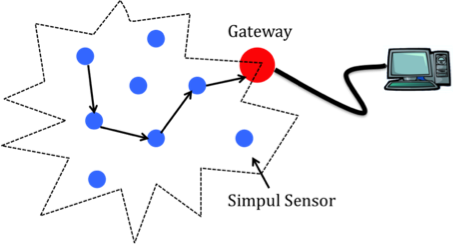
\includegraphics{gambar/wsn}
	\caption{Jaringan sensor nirkabel.}
	\label{wsn}
\end{figure}

 
%-----------------------------------------------------------------


\end{document}